\documentclass[tikz,border=6pt]{standalone}
\usepackage{amsmath,amssymb}
\usepackage{xcolor}
\definecolor{accent}{HTML}{A13D2C}
\definecolor{accent2}{HTML}{2B5F6B}
\definecolor{muted}{HTML}{5A564F}
\definecolor{panel}{HTML}{F8F6F0}
\definecolor{linecol}{HTML}{D8D2C4}
\definecolor{sunyellow}{HTML}{E8A33D}
\definecolor{ink}{HTML}{1E1C1A}
\definecolor{colthree}{RGB}{60,140,80}
\usetikzlibrary{calc,arrows.meta,plotmarks}
\IfFileExists{results/ch6/timing_peg.dat}{\def\datadir{results/ch6/}}{\def\datadir{../results/ch6/}}
\usepackage[T1]{fontenc}\usepackage{newpxtext,newpxmath}  % same fonts as the notes
\begin{document}
% Timing curves computed from published orbits, code/ch6/02_timing.py.
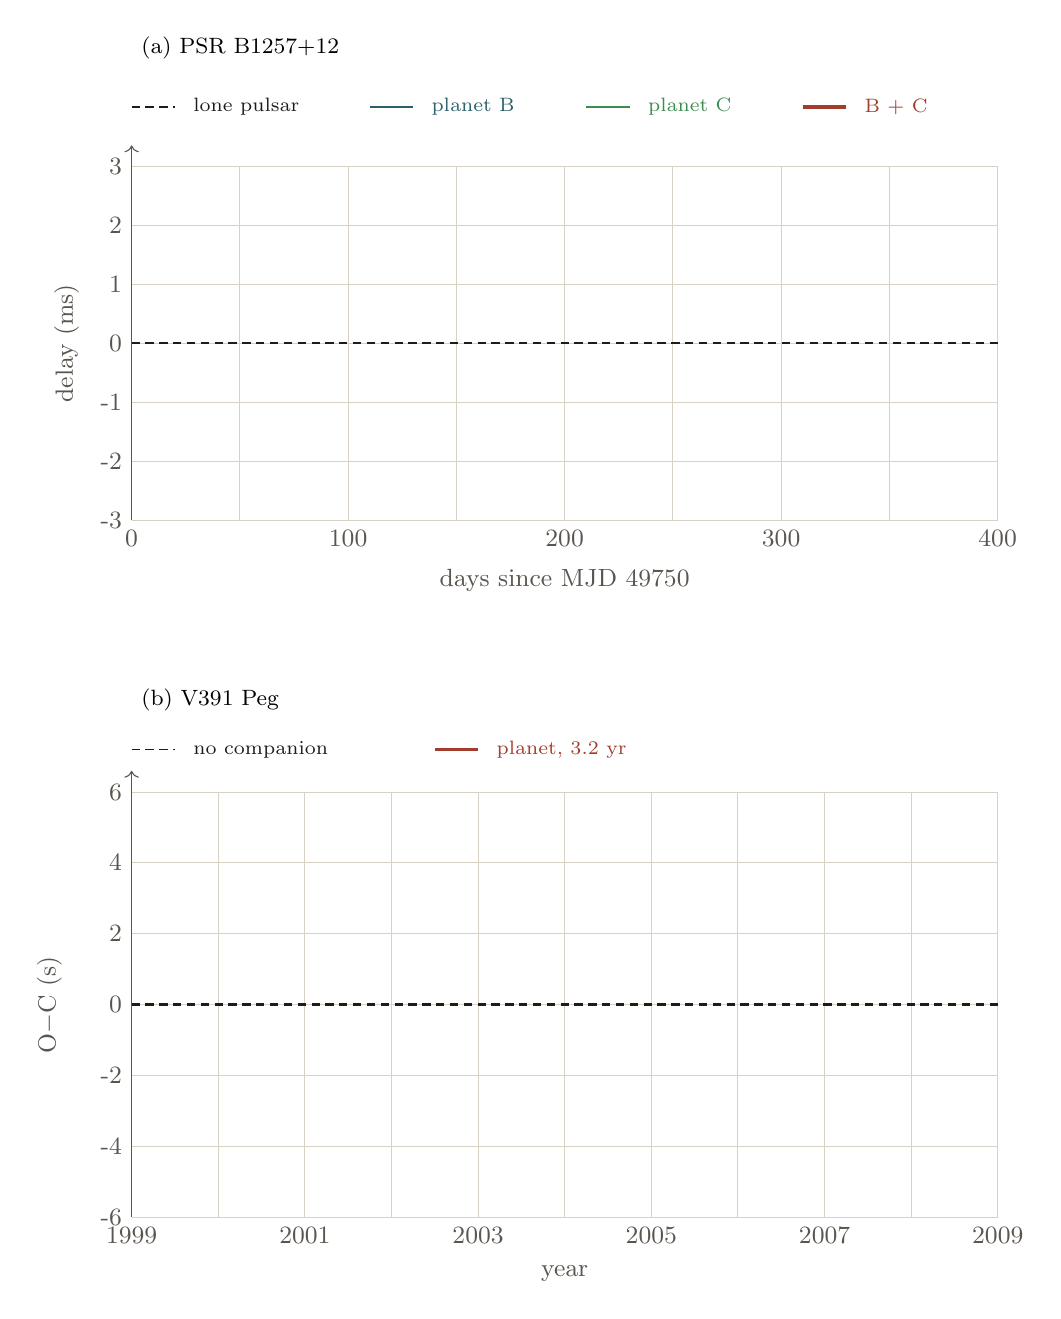
\begin{tikzpicture}[font=\small]
  % ---- (a) PSR B1257+12, x = 0.0275 cm/day, y = 0.75 cm/ms ----
  \begin{scope}[x=0.0275cm,y=0.75cm]
    \draw[linecol] (0,-3) grid[xstep=50,ystep=1] (400,3);
    \draw[->, muted] (0,-3) -- (0,3.35);
    \node[muted, rotate=90] at (-30,0) {delay (ms)};
    \foreach \y in {-3,-2,-1,0,1,2,3} \node[left, muted] at (0,\y) {\y};
    \foreach \x in {0,100,200,300,400} \node[below, muted] at (\x,-3) {\x};
    \node[muted, below=14pt] at (200,-3) {days since MJD 49750};
    \draw[ink, line width=0.9pt, densely dashed] (0,0) -- (400,0);
    \draw[accent2, line width=0.6pt] plot file {\datadir timing_psr_B.dat};
    \draw[colthree, line width=0.6pt] plot file {\datadir timing_psr_C.dat};
    \draw[accent, line width=1.1pt] plot file {\datadir timing_psr_sum.dat};
    \node[anchor=west, font=\footnotesize] at (0,5.0) {(a) PSR B1257+12};
    \draw[ink, densely dashed] (0,4.0) -- (20,4.0); \node[ink, anchor=west, font=\scriptsize] at (24,4.0) {lone pulsar};
    \draw[accent2, line width=0.6pt] (110,4.0) -- (130,4.0); \node[accent2, anchor=west, font=\scriptsize] at (134,4.0) {planet B};
    \draw[colthree, line width=0.6pt] (210,4.0) -- (230,4.0); \node[colthree, anchor=west, font=\scriptsize] at (234,4.0) {planet C};
    \draw[accent, line width=1.1pt] (310,4.0) -- (330,4.0); \node[accent, anchor=west, font=\scriptsize] at (334,4.0) {B + C};
  \end{scope}
  % ---- (b) V391 Peg, x = 1.1 cm/yr, y = 0.45 cm/s ----
  \begin{scope}[shift={(0,-8.4cm)}, x=1.1cm,y=0.45cm]
    \draw[linecol] (0,-6) grid[xstep=1,ystep=2] (10,6);
    \draw[->, muted] (0,-6) -- (0,6.6);
    \node[muted, rotate=90] at (-0.95,0) {O$-$C (s)};
    \foreach \y in {-6,-4,-2,0,2,4,6} \node[left, muted] at (0,\y) {\y};
    \foreach \x/\l in {0/1999,2/2001,4/2003,6/2005,8/2007,10/2009} \node[below, muted] at (\x,-6) {\l};
    \node[muted, below=14pt] at (5,-6) {year};
    \draw[ink, line width=0.9pt, densely dashed] (0,0) -- (10,0);
    \draw[accent, line width=1.1pt] plot file {\datadir timing_peg.dat};
    \node[anchor=west, font=\footnotesize] at (0,8.6) {(b) V391 Peg};
    \draw[ink, densely dashed] (0,7.2) -- (0.5,7.2); \node[ink, anchor=west, font=\scriptsize] at (0.6,7.2) {no companion};
    \draw[accent, line width=1.1pt] (3.5,7.2) -- (4,7.2); \node[accent, anchor=west, font=\scriptsize] at (4.1,7.2) {planet, 3.2 yr};
  \end{scope}
\end{tikzpicture}
\end{document}
